\section*{Backup Section}
This is the content of the backup section that won't appear in the Table of Contents.

\begin{frame}{Problems of LLMs}
    \begin{columns}[T]
        \begin{column}{0.70\textwidth}
            The works aimed at correcting LLMs can be classified according to the issues they tackle:
            \begin{enumerate}
                \item Hallucination: plausible-sounding but false information~\cite{gao2023rarr, zhang2023language}.

                \item Unfaithful Reasoning: derived conclusion does not follow the previously generated reasoning chain~\cite{he2022rethinking, pan2023logiclm}.

                \item Toxic Contents: content that is toxic, biased, or harmful due to biases present in the training datas~\cite{lu2022quark, gou2023critic}.

                \item Flawed Codes: flawed or incorrect code generation~\cite{chen2023teaching, olausson2023selfrepair}.
            \end{enumerate}
        \end{column}
        \begin{column}{0.30\textwidth}
            \begin{figure}[!htb]
                \centering
                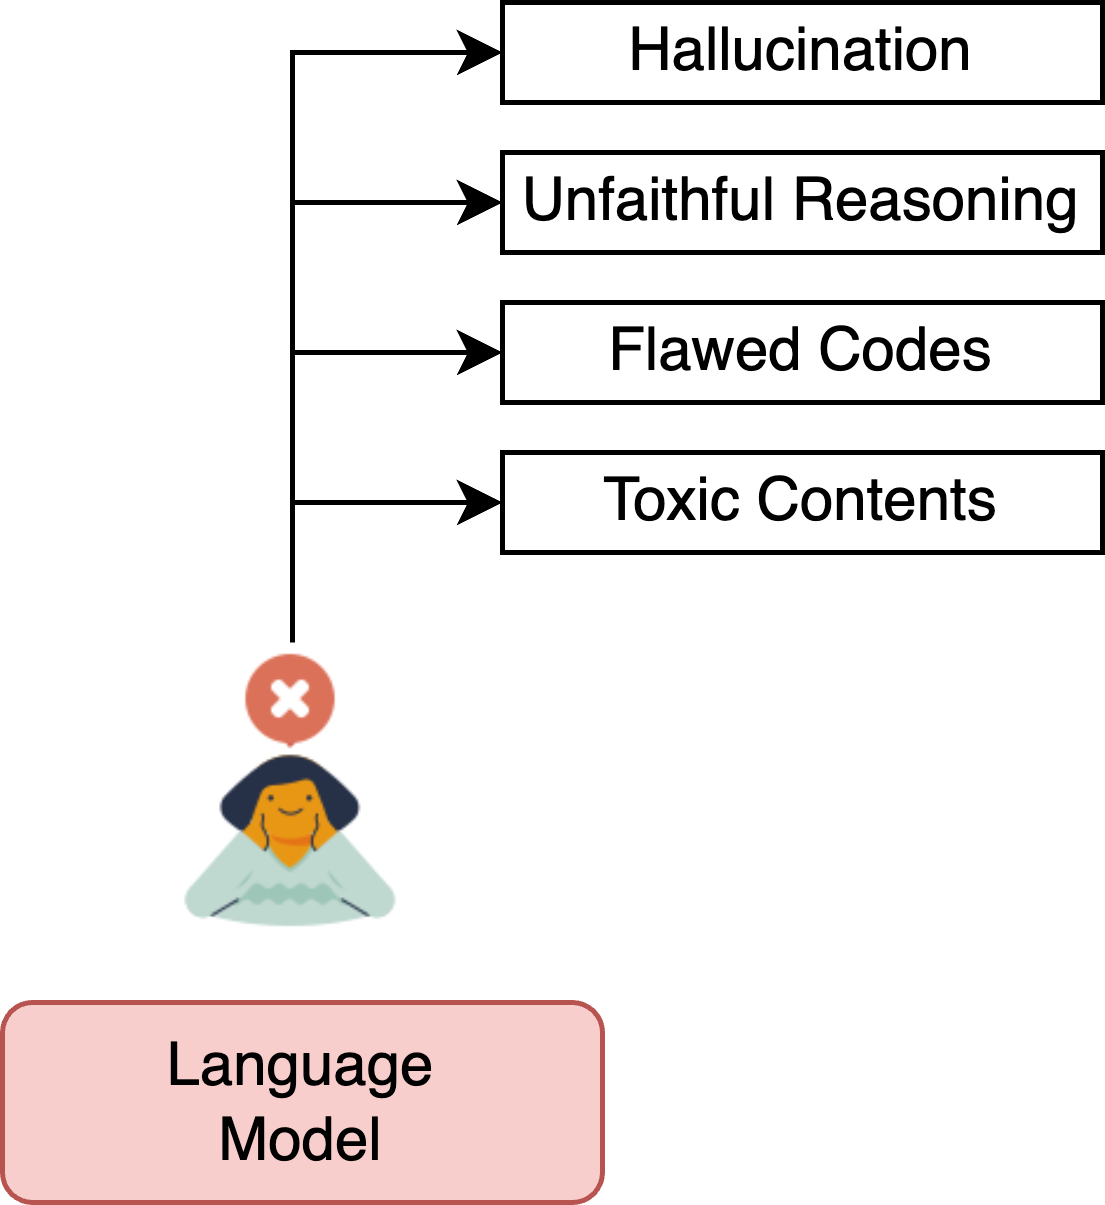
\includegraphics[width=1\textwidth]{img/language_model}
                \captionsetup{font=small,labelformat=empty}
                \caption{Problems of LLMs.}
            \end{figure}
        \end{column}
    \end{columns}
\end{frame}

\begin{frame}{Critic Model}
    \begin{columns}[T]
        \begin{column}{0.55\textwidth}
            Source of feedback:
            \begin{enumerate}
                \item Self-Feedback: the model itself generates feedback~\cite{weng2023large}.

                \item External Feedback: the model receives feedback from an external source (e.g., human, program executor and external knowledge)~\cite{gou2023critic}.
            \end{enumerate}

            Format of feedback:
            \begin{enumerate}
                \item Scalar Value: metrics based on pre-defined tests~\cite{weng2023large}.

                \item Natural Language: provides richer information than scalar value feedback~\cite{chen2023teaching}.
            \end{enumerate}
        \end{column}
        \begin{column}{0.45\textwidth}
            \begin{figure}[!htb]
                \centering
                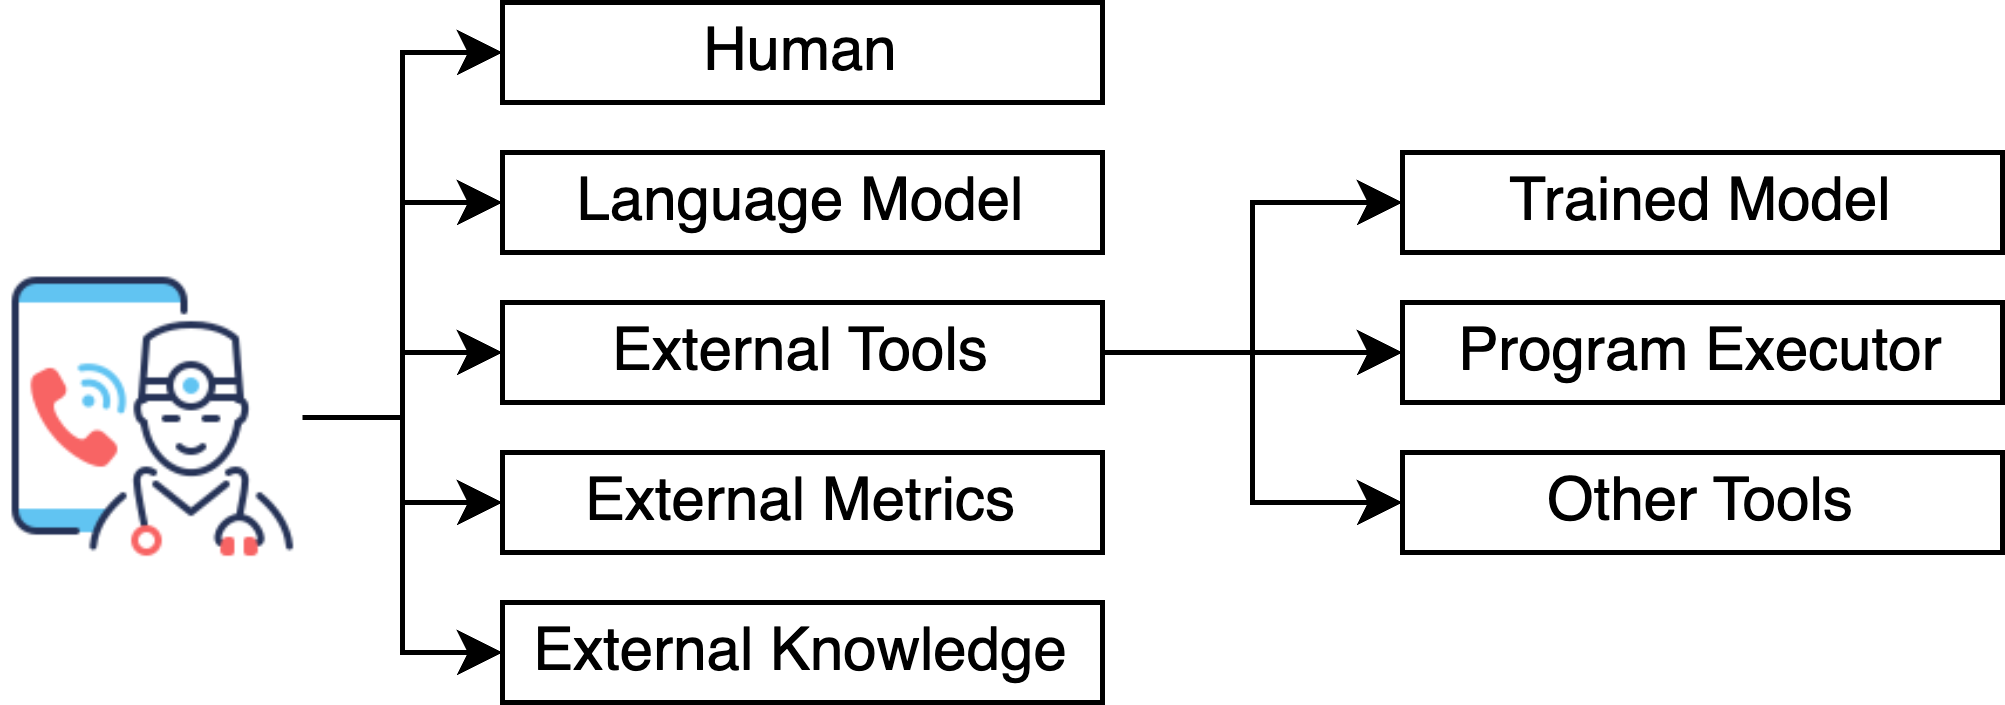
\includegraphics[width=1\textwidth]{img/critic_model}
                \captionsetup{font=small,labelformat=empty}
                \caption{Critic Model.}
            \end{figure}
        \end{column}
    \end{columns}
\end{frame}

\begin{frame}[fragile]{Example: Pandas-273 Problem}
    \begin{verbatim}
Problem:
I do know some posts are quite similar to my question but none of them succeeded in giving me the correct answer. I want, for each row of a pandas dataframe, to perform the sum of values taken from several columns. As the number of columns tends to vary, I want this sum to be performed from a list of columns.
At the moment my code looks like this:
df['Sum'] = df['Col A'] + df['Col E'] + df['Col Z']

I want it to be something like:
df['Sum'] = sum(list_of_my_columns)

or
df[list_of_my_columns].sum(axis=1)

But both of them return an error. Might be because my list isn't properly created? This is how I did it:
list_of_my_columns = [df['Col A'], df['Col E'], df['Col Z']]

But this doesn't seem to work... Any ideas? Thank you!
    \end{verbatim}
\end{frame}

\begin{frame}[fragile]{Example: Pandas-273 CoT Prompt}
    \begin{verbatim}
Here are the step-by-step suggestions to guide CoT-SelfEvolve
to solve the problem:
Suggestion 1: Understand the problem requirements: The goal
is to calculate the sum of values from multiple columns
in a pandas DataFrame, where the column names are stored in
a list.
Suggestion 2: Review the given code and identify the issue:
The current code `list_of_my_columns = [df['Col A'],
df['Col E'], df['Col Z']]` is incorrect because it's creating
a list of Series objects, not a list of column names.
Instead, create a list of column names as strings, like
`list_of_my_columns = ['Col A', 'Col E', 'Col Z']`.
By following these suggestions, CoT-SelfEvolve should be able
to solve the problem and calculate the sum of values from
multiple columns in the pandas DataFrame.
    \end{verbatim}
\end{frame}

\begin{frame}[fragile]{Example: Pandas-273 Solution}
    \begin{verbatim}
import pandas as pd
import numpy as np

df, list_of_my_columns = \
pickle.load(open(f"input/input{args.test_case}.pkl", "rb"))

###BEGIN SOLUTION
df['Sum'] = df[list_of_my_columns].sum(axis=1)
###END SOLUTION

result = df

with open('result/result_{}.pkl'.format(
    args.test_case), 'wb') as f:
    pickle.dump(result, f)
    \end{verbatim}
\end{frame}
